%!TEX TS-program = XeLaTeX
\documentclass[12pt]{article}
\usepackage[top=1in, bottom=1in, left=1in, right=1in]{geometry}

%%%
%% Needed for fonts in xelatex to work
%%%
% NOTE: I actually use XeLaTeX, which allows me to get the fonts
% exactly the way that I want them. For proposals, this means
% I can use Times New Roman instead of the default Computer
% Modern. I actually like Computer Modern, but since Arial
% is what the solicitation suggests there's no point in throwing off a reviewer
% with an unexpected font, particularly one with such a
% polarizing reaction in readers. Never upset the reviewrers, I
% always say.
%
% What's the point of this bit of rambling? If you do not want to use
% XeLaTeX and would rather stick to good old LaTeX, then you
% need to comment out the next few lines of font packages and
% font commands.
%
% If you want to use XeLaTeX but want different fonts, then you
% just need to change the name in the argument for \setmainfont.
% Make sure that the font you use is loaded on
% your machine and your TeX distribution knows how to find it.
% See Google if you need to learn more about this.
%
\usepackage{fontspec}
\setmainfont{Arial}

%%%
%% Packages that I use on a regular basis.
%%%
% Of course, you are likely to need some math typesetting so these
% three packages have you covered.
\usepackage{amssymb}
\usepackage{amsmath}
\usepackage{latexsym}
% I use color, graphicx, and epstopdf to read in PDFs for my figures.
\usepackage{color}
\usepackage{graphicx}
\usepackage{epstopdf}
% I don't remember why threeparttable and setspace is here. Inertia.
\usepackage{threeparttable}
\usepackage{setspace}
%%%
%% Some packages to handle the figures and captions
%%%
\usepackage[labelfont=bf]{caption}
\usepackage{subcaption}
\usepackage{wrapfig}

%%%
%% Packages and settings for my bibliography.
%%%
% apa_with_doi is a style I created to keep DOI in the bibliography
% but strip out URLs. There are a lot of other styles you can
% find for natbib. Again, Google is your friend.
% Author name and year references, i.e., Author (year):
%\usepackage{natbib}
%\bibliographystyle{apa_with_doi}
% Numbered references:
\usepackage[numbers,super]{natbib}
\bibliographystyle{unsrtnat}


%%%
%% Packages and commands to build my table of contents (TOC).
%%%
%% The trick was getting the References included properly.
%% Also, some of my table of contents entry have no page number
%% because those pages are generated separately by my institute.
%% Nothing to be done about that. You may or may not have the
%% same problem, so you may or may not have to tweak this.
\usepackage[nottoc,numbib]{tocbibind}
\renewcommand{\tocbibname}{References}
\usepackage{tocloft}
\renewcommand{\cftsecleader}{\cftdotfill{\cftdotsep}}

%%%
%% These commands get the spacing around the title and section titles right.
%%%
% I tightened up the spacing. The LaTeX default is just too roomy.
% This spacing is still clean and legible, just not so free with the
% whitespace between sections.
%
% First the title.
\usepackage{titling}
\setlength{\droptitle}{-50pt}
\pretitle{\begin{center}\Large\bfseries\vspace{0ex}}%
\posttitle{\end{center}\Large\vspace{-2ex}}%
\preauthor{\begin{center}\large}%
\postauthor{\end{center}\large\vspace{-3ex}}%
\predate{\begin{center}\large}%q
\postdate{\end{center}\large\vspace{-6ex}}%
% Now the section headings.
\usepackage[noindentafter]{titlesec}
\titleformat{\section}{\large\bfseries}{\thesection}{1em}{}
\titlespacing{\section}{0pt}{18pt plus 2pt minus 2pt}{4pt plus 2pt minus 2pt}[0pt]
\titlespacing{\subsection}{0pt}{16pt plus 2pt minus 2pt}{4pt plus 2pt minus 2pt}[0pt]
\titlespacing{\subsubsection}{0pt}{14pt plus 2pt minus 2pt}{4pt plus 2pt minus 2pt}[0pt]

%%%
%% These commands get the lists to work the way that I want them to.
%%%
% i.e. I want less space wrapping around the list.
\usepackage{enumitem}
\setlist{nolistsep}
\setlist[2]{noitemsep}
\setlist[1]{noitemsep}

%%%
%% Commands for making the tables.
%%%
\usepackage{booktabs}
\usepackage{multirow}
\usepackage{array}


%%%
%%% Formatting urls
%%%
\usepackage{url}
\urlstyle{rm}

%% The lineno packages adds line numbers. Start line numbering with
%% \begin{linenumbers}, end it with \end{linenumbers}. Or switch it on
%% for the whole article with \linenumbers after \end{frontmatter}.
\usepackage{lineno}

%% In order to have a caption to the side of a figure or table, use the
%% 'sidecap' package.
\usepackage[rightcaption]{sidecap}
\sidecaptionvpos{figure}{t}

\usepackage{wrapfig}


%% For more control of the enumeration environment (lists with numbers)
%% use the enumitem package.
%\usepackage{enumitem}

%% Also, to reset the numbering of enumerate, use the following:
%\setenumerate[0]{label=\alph*.}

% To deal with figures all alone on a page.
\renewcommand{\floatpagefraction}{.8}%

% To use symbols for the footnotes:
\renewcommand{\thefootnote}{\fnsymbol{footnote}}

% set up the page numbers as 1-N, 2-N, ...
\numberwithin{page}{section}
\renewcommand{\thepage}{\thesection-\arabic{page}}

% https://tex.stackexchange.com/questions/210871/latex-page-numbering-by-section
%this does not seem to work, just hard code it :(
% not sure if there is something else in this template that is breaking it
% or things have changed in the last 6 years?
%\usepackage{etoolbox}
%\makeatletter
%% Make sure that page starts from 1 with every \section
%\patchcmd{\@sect}% <cmd>
%  {\protected@edef}% <search>
%  {\def\arg{#1}\def\arg@{section}%
%   \ifx\arg\arg@\stepcounter{page}\fi%
%   \protected@edef}% <replace>
%  {}{}% <success><failure>
%\makeatother

%% Finally, we get to the document.
\begin{document}
\title{Improving the Foundations and Maintenance of Matplotlib and CartoPy}
\author{Dr. Thomas A Caswell\\Dr. Ryan May}
\date{}
\maketitle

% First, let's get that TOC in there. NASA likes it.
\setcounter{tocdepth}{2}
\tableofcontents
\thispagestyle{empty}
% Let's leave this TOC alone on this page and start a new one for
% proposal body.
\newpage

\section{Scientific/Technical/Management (S/T/M)}
% Let's reset the page counter.
\setcounter{page}{1}
% the subsection are a combination of the lines labeled "Content" in
% Table 1 (on ROSES-20 SoS-51) and the text in E.7.3 (on E.7-2 -
% E.7-3) describing what needs to be in the proposal.

% not sure that this order is right, but I think we need to hit all of
% these points.  Maybe want to rename the section headings or merge
% some of them?
\subsection{description of software and relevance to SMD}

Matplotlib\cite{Hunter:2007} is the fundamental data visualization
library for the scientific Python Ecosystem, used in conjunction with
other foundational tools like NumPy\cite{Harris2020},
SciPy\cite{Virtanen2020}, and pandas.  This ecosystem, shown with a
rough schematic in Figure \ref{fig:ecosystem}, has a core of general
purpose domain-agnostic tools with concentric rings of increasingly
domain specific tools.  This layered approach gives scientists both
convenient high level tools and direct access to the underlying
libraries when needed.

CartoPy is a Matplotlib extension library that brings support for
mapping applications to Matplotlib, providing support for plotting
using a variety of map projections (both terrestrial and non) as well
as providing out-of-the-box support for many terrestrial map
features. CartoPy is currently the only Matplotlib-based plotting
library for mapping applications being actively developed in the
Python ecosystem. CartoPy is frequently used for earth science
applications, including many uses of NASA Earth science datasets.

\begin{wrapfigure}{r}{0.5\textwidth}
  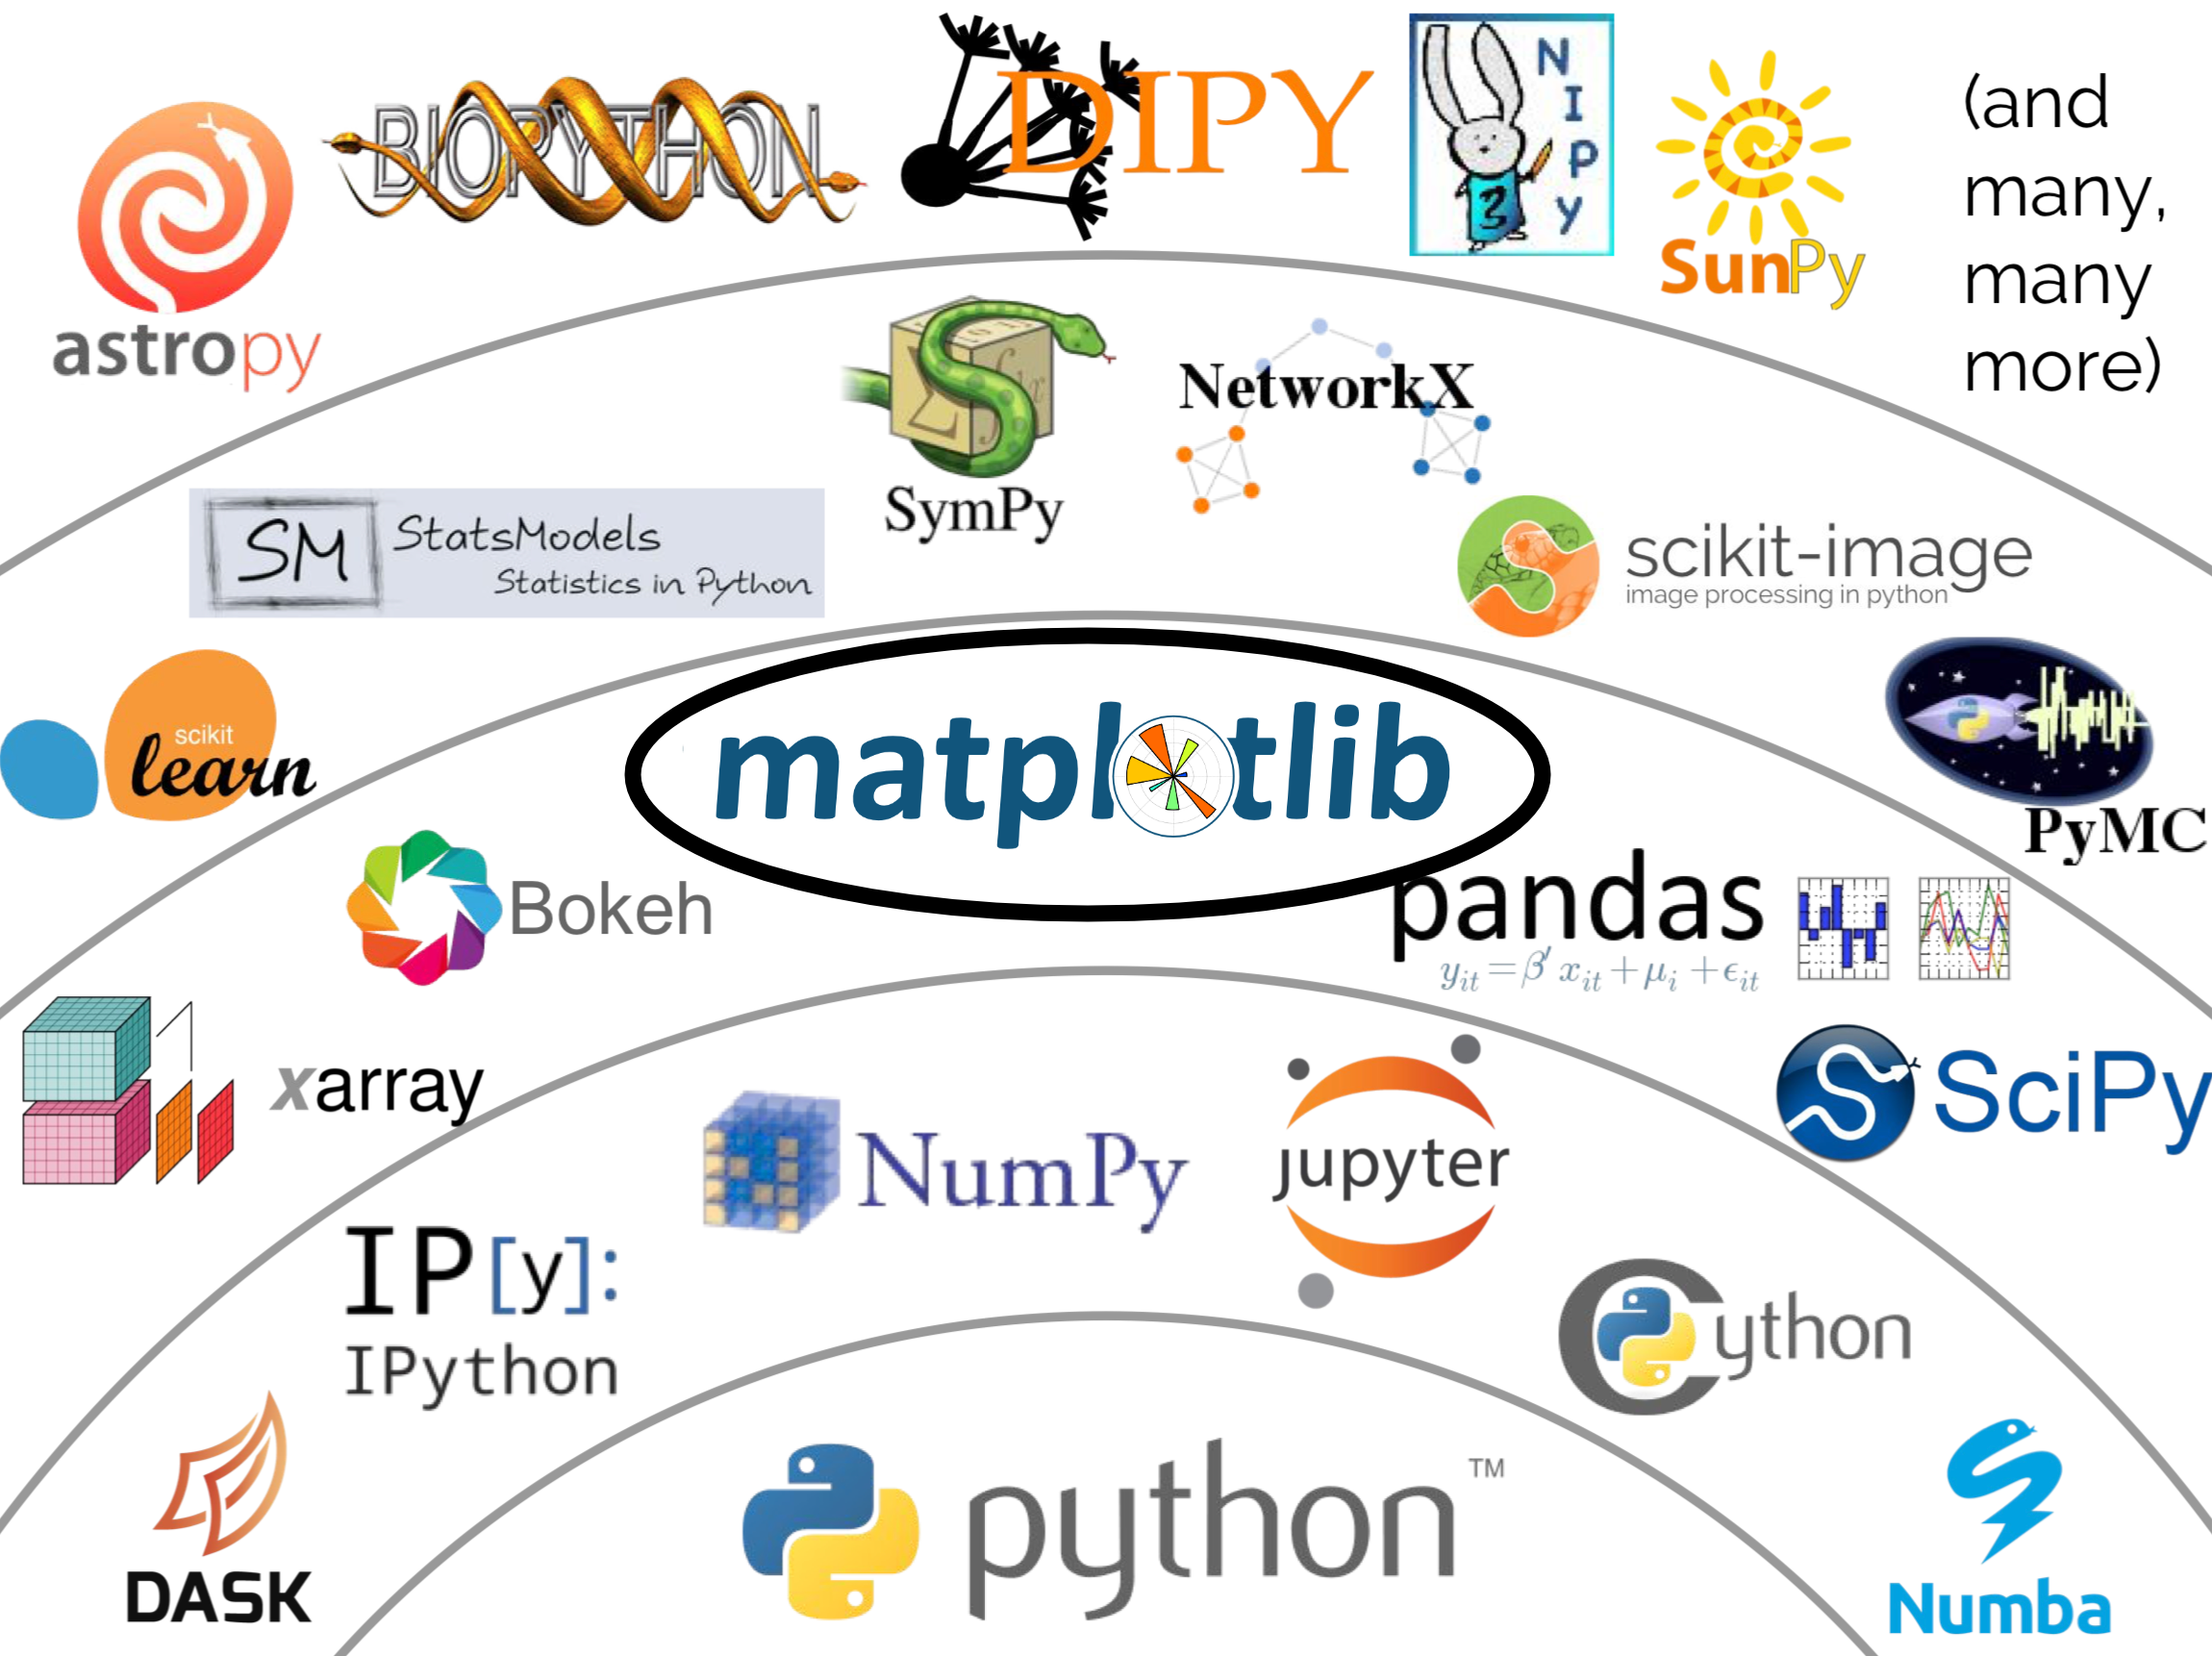
\includegraphics[width=0.45\textwidth]{scipy-ecosystem}
  \caption{A schematic of the Scientific Python ecossytem.  At the
    center we have the Python language itself with concentric rings of
    domain agnostic to domain specific libraries.  Both astropy (top
    left) and sunup (top right), for arstropyhsics and heiophysics
    respectively both rely on Matplotlib. Cartopy, which is not shown,
    would be placed in the outer [CHECK] ring.  Credit: Jake van der
    Plas, "The Unexpected Effectiveness of Python in Science", PyCon
    2017}
  \label{fig:ecosystem}
\end{wrapfigure}


The initial commits in the Matplotlib history date to early 2003 and
the initial work was done in 2001-2002. Matplotlib has been actively
developed and maintained by a vibrant, primarily volunteer, community
over the last 17 years.  Matplotlib has over 1,000 individual
contributors to the code base, estimated to have over a million users,
is in top 100 most downloaded Python packages from pypi, and is packaged
by every major linux distribution.

The most common visualizations in a domain need to be fluid for the
end-practitioners, with the ``obvious'' customization options
exposed. Much of the domain-specific specialization is carried in the
structure, semantics and assumptions of the data, and in the standard
visualizations of the domain. These specializations can vary widely,
in contradictory ways, between domains. Because no high-level API can
simultaneously satisfy all of the visualization needs, there has
developed a rich ecosystem of domain specific plotting tools including
including yt, astropy, ArviZ, xarray, cartopy, astropy,
fast\_histogram, and metpy [tune to be more NASA specific?].

Matplotlib \cite{Hunter:2007} is an established open source plotting
library with a BSD-derived license that is currently used through out
both the SMD science community and the wider scientific community for
both publication quality figures and for

Matplotlib has an API for both quick plotting, as required from
exploratory data analysis, and an API that gives full control the
visualization for fine-tuning plots for publication.  Matplotlib also
provides a framework to develop GUI independent interactive data
exploration tools and animation.



\subsection{Objectives and Significance}
\subsubsection{Unit work}

Matplotlib supports plotting unit-aware data structures which have
been used to support spaceflight operations by Monte, JPL's mission
design and navigation software system. Initial development of this
capability was supported by NASA. However, this support is under
documented making it difficult for users to understand how to fully
make use of the capability. Further, because we do not have full test
coverage of all plotting functions to verify that they correctly
handle units we have had a number of regressions in the
functionality. We will propose to write thorough user and technical
guides to working with unit-aware data in Matplotlib, add 100\% test
coverage of unit support in our plotting routines, and fix any issues
and inconsistencies discovered in this process.

\subsubsection{Cartopy guts}
CartoPy's mapping capabilities leverages the widely-used PROJ library
for mapping projections and the GEOS library for geometry
applications. Currently, CartoPy maintains custom code to interface
Python with these C-based libraries. As part of this work, we propose
porting Cartopy to instead use existing libraries that provide Python
bindings for these libraries, PyPROJ and PyGEOS. Not only will this
reduce CartoPy's overall amount of code and enhance maintainability,
but it will also address two of the biggest challenges that occur in
packaging CartoPy for its user-base.

\subsubsection{General maintenance}

Matplotlib and Cartopy are community-driven projects, but we have
grown to the point where we need developers with the time to organize,
plan, and make decisions.

Pull Requests (PRs) and Issues are submitted faster than they can be
reviewed; Matplotlib has accumulated about 300 open PRs 1300 open
Issues due to this imbalance, while CartoPy currently stands at 40
open PRs and 229 open Issues.  This imbalance is not due lack of
activity, in 2020 Matplotlib resolved 125-200 PRs and 75-125 Issues a
month but only reduced the PR backlog by 70 open PRs and making no progress
on reducing the Issue backlog.

There may be critical bug reports or insightful feature requests among
the former, while among the latter are useful contributions or bug
fixes that would improve the libraries for direct users and downstream
packages.  The backlog is discouraging for new and occasional
contributors and distracting for core developers. The resources we
will request will help to significantly reduce, but not eliminate,
this backlog.

To maintain Matplotlib's and Cartopy's health we need to:
%% these can probably be shortened further, to just stuff like Triage and on board
%%since explainations are in text
\begin{itemize}[noitemsep]
\item fix critical bugs and regressions;
\item triage the backlog of Issues and PRs in terms of topic, difficulty, and urgency and promptly triage newly opened Issues and PRs;
\item maintain backward compatibility and extensively document intentional changes;
\item on-board new contributors to sustain and diversify developer team;
\item and manage discussions about proposed enhancements, features, and API changes.
\end{itemize}

The requested support for developers is intended to complement and
facilitate, not replace, crucial volunteer work.  We aim to better
co-ordinate and nurture their efforts, with the goal of growing and
sustaining a diverse community of volunteer and paid expert
contributors.

\subsection{Perceived impact of work}
\begin{enumerate}
\item increased reliability of unit-aware plotting
\item improvement in general reliability of software
\item improved responsively to issues
  \begin{enumerate}
  \item in 2020 have had paid developer for 9mo
  \item making progress on PRs, holding steady on issues
  \end{enumerate}
\item easier installation and deployment
\end{enumerate}
\subsection{Relevance to program element}

TODO make this flow...at all...

Matplotlib is used through out all of the program elements of the SMD.
In Earth observation Matplotlib has been used to study thunderstorms
\cite{https://doi.org/10.1002/2016JD025299,https://doi.org/10.1029/2019JD030874},
seasonal ocean winds \cite{https://doi.org/10.1002/2017JD027516} and
tropical storms \cite{Lang_2020}.  Matplotlib was used in the first
science paper from the Parker Solar probe\cite{Bale2019}.  Matplotlib
has been used as part of the Martian science program in both an
orbiter \cite{https://doi.org/10.1029/2019JE006188} and
rover\cite{https://doi.org/10.1002/2016EA000219} contexts.
Historically, Matplotlib was used as part of ground operations from
the Phoenix Lander.  Matplotlib was used on data from Kepler and K2
missions to study Trojan asteroids\cite{Nixon_2019} and Titan
\cite{Ryan_2017,2019PASP..131h4505P}.
Matplotlib is used for visualization of scheduling, safety+constraint checks, and telemetry by the Swift science operations team \cite{swift_ops,2020ApJ...900...35T}.
Both the Hubble and James Web Space Telescopes data processing
developed by Space Telescope Science Institute rely on Matplotlib [CITE NEEDED].
Matplotlib is used to support spaceflight operations by Monte, JPL's
mission design and navigation software system [CITE NEEDED].
Matplotlib is being used in the New Horizons Kuiper belt extended mission \cite{Porter_2018}.  Matplotlib
has been used for fundamental research on graphene \cite{PhysRevLett.120.236802} and
work on nuclear rockets \cite{leu_cerment}.

Need more examples of SMD using Cartopy!

Matplotlib supports plotting unit-aware data structures which have
been used to support spaceflight operations by Monte, JPL's mission
design and navigation software system. (TODO expand this!)

\subsection{Technical approach and methodology}

our standard practice!

\subsection{sources of uncertainty}

Units and cartopy overhaul may be more work than expected when we start digging in.

Maintenance is low risk, we know there is a pile of small tasks to be
done than can be reduced by applying effort.  Have demonstrated that
paid developers helps.

\subsection{mitigation to risk}

Will not regress from functional status quo, all work will be an
improvement but maybe not as much as we plan for.

\subsection{roles of team members}
\begin{enumerate}
\item Caswell: PI + maintenance + community/governance work
\item May: Cartopy refactor + unit expertise + maintenance
\item RSE: maintenance + lead unit unit testing
\end{enumerate}

\subsection{workplan with milestones}

\subsection{Project Management}
\subsubsection{Governance}
Matplotlib is a NumFOCUS Fiscally Sponsored Project.  The governance
is specified by
\url{https://github.com/matplotlib/governance/blob/master/governance.md}.
The project has a Project Lead (Caswell) who is the final authority in
all decisions, however when possible all decisions are made by
community consensus.  In addition to the Project Lead, there is a
formalized Steering Council which is responsible for the overall
direction of the project, and several Deputy Project Leads who have
day-to-day technical responsibilities.



\subsubsection{License}

BSD-derived and LGPL

\subsubsection{sustainability metrics}
\begin{enumerate}
\item Continue Regular releases (mpl minor every 6mo, patch every 2mo
  or as needed).
\item Increase number of new regular contributors
\item Total number of outstanding open PRs / Issues reduced
\end{enumerate}

\subsubsection{collaboration with related projects}
Matplotlib has well established relationships with both up and
downstream projects.

The strongest relationships, both historical and current, are with
projects where we have shared developers.  For example Ryan May and
Elliot sales de Andre are both core contributors to Matplotlib and
Cartopy.  Micheal Droettboom, the previous Matplotlib Project lead,
was also a core developer on Astropy.  Almost all of the Matplotlib
contributors are expert Matplotlib users in their primary science
domain.

We maintain multiple communication channels with related projects.
These include on-line communication, such as reporting issues to each
other's issue trackers, asking questions on mailing lists or
discussions forums, and submitting patches.  Inter-project
relationships are also facilitated by meetings and conferences
organized by NumFOCUS.



\subsubsection{inclusive practices}

Matplotlib strives to be an inclusive and open project and have
adopted a Code of Conduct
\url{https://github.com/matplotlib/matplotlib/blob/master/CODE_OF_CONDUCT.md}. Anyone
who is willing to contribute to the project should be able to do.  It
is important for everyone working on the project to feel safe to make
mistakes.

One challenge of being an open community developed project is that we do not
have reliable demographics on a vast majority of our contributors.

We have recently started two efforts to improve the development and
retention of new contributors: an ``incubator'' channel on gitter and
a Triage Team.

The hardest part of getting started to contributing to open source
projects is can be simply getting started.  The incubator is a
semi-closed chat room where new contributors can get support on any
aspect of contributing to Matplotlib.  This include the technical
aspects of the code they are working on, help with git/github, our
review process, or the social expectations and norms of the community.  The
goal is that by providing this support to first time contributors we will
retain more of them as regular contributors and then maintainers.

The issue tracker is important to communication in the project because
it serves as the centralized location for making feature requests,
reporting bugs, identifying major projects to work on, and discussing
priorities.  For this reason, it is important to curate the issue
list, adding labels to issues and closing issues that are resolved or
unresolvable. Triaging issues does not require any particular
expertise in the internals of Matplotlib but is extremely valuable to
the project.  To this end we have created a ``Triage Team'' in the
organization who have power to tag, milestone, and close issues.  In
addition to the direct benefit of improving the issue triage and
freeing the core-developers to spend more time reviewing PRs, this
role will bring more people into the developer community and may
provide a path way to becoming regular contributors and maintainers.


We will work with NumFOCUS to develop metrics and evaluate the efficacy of
these efforts at diversifying our contributor base.

\subsubsection{information dissemination}
\begin{enumerate}
\item docs
\item github
\item discourse
\item mailing lists
\item pydata events
\item twitter
\end{enumerate}

\subsection{describe current workflow}

\newpage
\setcounter{page}{1}
% Here's how I get references.
% needed for AAS citation

\def\ref@jnl#1{{\rm#1}}

\def\aj{\ref@jnl{AJ}}                   % Astronomical Journal
\def\actaa{\ref@jnl{Acta Astron.}}      % Acta Astronomica
\def\araa{\ref@jnl{ARA\&A}}             % Annual Review of Astron and Astrophys
\def\apj{\ref@jnl{ApJ}}                 % Astrophysical Journal
\def\apjl{\ref@jnl{ApJ}}                % Astrophysical Journal, Letters
\def\apjs{\ref@jnl{ApJS}}               % Astrophysical Journal, Supplement
\def\ao{\ref@jnl{Appl.~Opt.}}           % Applied Optics
\def\apss{\ref@jnl{Ap\&SS}}             % Astrophysics and Space Science
\def\aap{\ref@jnl{A\&A}}                % Astronomy and Astrophysics
\def\aapr{\ref@jnl{A\&A~Rev.}}          % Astronomy and Astrophysics Reviews
\def\aaps{\ref@jnl{A\&AS}}              % Astronomy and Astrophysics, Supplement
\def\azh{\ref@jnl{AZh}}                 % Astronomicheskii Zhurnal
\def\baas{\ref@jnl{BAAS}}               % Bulletin of the AAS
\def\bac{\ref@jnl{Bull. astr. Inst. Czechosl.}}
                % Bulletin of the Astronomical Institutes of Czechoslovakia
\def\caa{\ref@jnl{Chinese Astron. Astrophys.}}
                % Chinese Astronomy and Astrophysics
\def\cjaa{\ref@jnl{Chinese J. Astron. Astrophys.}}
                % Chinese Journal of Astronomy and Astrophysics
\def\icarus{\ref@jnl{Icarus}}           % Icarus
\def\jcap{\ref@jnl{J. Cosmology Astropart. Phys.}}
                % Journal of Cosmology and Astroparticle Physics
\def\jrasc{\ref@jnl{JRASC}}             % Journal of the RAS of Canada
\def\memras{\ref@jnl{MmRAS}}            % Memoirs of the RAS
\def\mnras{\ref@jnl{MNRAS}}             % Monthly Notices of the RAS
\def\na{\ref@jnl{New A}}                % New Astronomy
\def\nar{\ref@jnl{New A Rev.}}          % New Astronomy Review
\def\pra{\ref@jnl{Phys.~Rev.~A}}        % Physical Review A: General Physics
\def\prb{\ref@jnl{Phys.~Rev.~B}}        % Physical Review B: Solid State
\def\prc{\ref@jnl{Phys.~Rev.~C}}        % Physical Review C
\def\prd{\ref@jnl{Phys.~Rev.~D}}        % Physical Review D
\def\pre{\ref@jnl{Phys.~Rev.~E}}        % Physical Review E
\def\prl{\ref@jnl{Phys.~Rev.~Lett.}}    % Physical Review Letters
\def\pasa{\ref@jnl{PASA}}               % Publications of the Astron. Soc. of Australia
\def\pasp{\ref@jnl{PASP}}               % Publications of the ASP
\def\pasj{\ref@jnl{PASJ}}               % Publications of the ASJ
\def\rmxaa{\ref@jnl{Rev. Mexicana Astron. Astrofis.}}%
                % Revista Mexicana de Astronomia y Astrofisica
\def\qjras{\ref@jnl{QJRAS}}             % Quarterly Journal of the RAS
\def\skytel{\ref@jnl{S\&T}}             % Sky and Telescope
\def\solphys{\ref@jnl{Sol.~Phys.}}      % Solar Physics
\def\sovast{\ref@jnl{Soviet~Ast.}}      % Soviet Astronomy
\def\ssr{\ref@jnl{Space~Sci.~Rev.}}     % Space Science Reviews
\def\zap{\ref@jnl{ZAp}}                 % Zeitschrift fuer Astrophysik
\def\nat{\ref@jnl{Nature}}              % Nature
\def\iaucirc{\ref@jnl{IAU~Circ.}}       % IAU Cirulars
\def\aplett{\ref@jnl{Astrophys.~Lett.}} % Astrophysics Letters
\def\apspr{\ref@jnl{Astrophys.~Space~Phys.~Res.}}
                % Astrophysics Space Physics Research
\def\bain{\ref@jnl{Bull.~Astron.~Inst.~Netherlands}}
                % Bulletin Astronomical Institute of the Netherlands
\def\fcp{\ref@jnl{Fund.~Cosmic~Phys.}}  % Fundamental Cosmic Physics
\def\gca{\ref@jnl{Geochim.~Cosmochim.~Acta}}   % Geochimica Cosmochimica Acta
\def\grl{\ref@jnl{Geophys.~Res.~Lett.}} % Geophysics Research Letters
\def\jcp{\ref@jnl{J.~Chem.~Phys.}}      % Journal of Chemical Physics
\def\jgr{\ref@jnl{J.~Geophys.~Res.}}    % Journal of Geophysics Research
\def\jqsrt{\ref@jnl{J.~Quant.~Spec.~Radiat.~Transf.}}
                % Journal of Quantitiative Spectroscopy and Radiative Transfer
\def\memsai{\ref@jnl{Mem.~Soc.~Astron.~Italiana}}
                % Mem. Societa Astronomica Italiana
\def\nphysa{\ref@jnl{Nucl.~Phys.~A}}   % Nuclear Physics A
\def\physrep{\ref@jnl{Phys.~Rep.}}   % Physics Reports
\def\physscr{\ref@jnl{Phys.~Scr}}   % Physica Scripta
\def\planss{\ref@jnl{Planet.~Space~Sci.}}   % Planetary Space Science
\def\procspie{\ref@jnl{Proc.~SPIE}}   % Proceedings of the SPIE

\let\astap=\aap
\let\apjlett=\apjl
\let\apjsupp=\apjs
\let\applopt=\ao

\bibliography{mpl_cartopy.bib}

\newpage
\section{Data Management Plan}
\setcounter{page}{1}

Matplotlib is a software library and does not produce any scientific
data as defined in E.1.2 that needs to be preserved.

Matplotlib is currently developed in the open on GitHub and is
released under a permissive license (the Matplotlib license which is a
derivative of the PSF license and compatible with BSD-3).  All work
done on Matplotlib as part of this grant will be done through the
current workflow, will be publicly available, and released under the
same license.  Matplotlib uses git for version control, thus every
developer has the full history on their computer which provides
significant redundancy.  Tagged releases of the software are published
to pypi (in both source and binary forms).  In addition, Anaconada,
macports, homebrew, and all major Linux distributions independently
build, package, and host Matplotlib.  User facing documentation is built
and hosted at \url{https://matplotlib.org}.

Cartopy is currently developed in the open on GitHub and is released
under the LGPL.  All work done on Matplotlib as part of this grant
will be done through the current workflow, will be publicly available,
and released under the same license. Cartopy uses git for version
control, thus every developer has the full history on their computer
which provides significant redundancy.

%do we need something about shape files / map tiles?

Any new libraries created as part of the ROSES award will be developed
in the open on GitHub and will released under a BSD-3 license.

% do we need this?
Any incidental work on other software packages, either upstream or
downstream of Matplotlib and Cartopy, will have to follow the license
and development of process of those projects, however precedence will
be given to OSS projects.


\newpage
\section{Biographical Sketches}
\setcounter{page}{1}
\newpage
\subsection{Principal Investigator}
\newpage
\subsection{Co-Investigator}

% This line gets the space in TOC right.
\addtocontents{toc}{\protect\vspace{12pt}}
\newpage
\section{Table of Personnel and Work Effort}
\setcounter{page}{1}

\newpage
\section{Current and Pending Support}
\setcounter{page}{1}

\newpage
\section{Budget Justification}
\setcounter{page}{1}

Due to being an established community driven project most regular
contributors have established and distinct primary institutions.  For
this reason significant portions of the budget will need to be
subcontracted to the primary institutions of key individuals who are
uniquely qualified for this work.

\newpage
\section{Facilities and Equipment}
\setcounter{page}{1}

None

\newpage
\section{Detailed Budget}
\setcounter{page}{1}



\end{document}
